\PassOptionsToPackage{unicode=true}{hyperref} % options for packages loaded elsewhere
\PassOptionsToPackage{hyphens}{url}
%
\documentclass[]{book}
\usepackage{lmodern}
\usepackage{amssymb,amsmath}
\usepackage{ifxetex,ifluatex}
\usepackage{fixltx2e} % provides \textsubscript
\ifnum 0\ifxetex 1\fi\ifluatex 1\fi=0 % if pdftex
  \usepackage[T1]{fontenc}
  \usepackage[utf8]{inputenc}
  \usepackage{textcomp} % provides euro and other symbols
\else % if luatex or xelatex
  \usepackage{unicode-math}
  \defaultfontfeatures{Ligatures=TeX,Scale=MatchLowercase}
\fi
% use upquote if available, for straight quotes in verbatim environments
\IfFileExists{upquote.sty}{\usepackage{upquote}}{}
% use microtype if available
\IfFileExists{microtype.sty}{%
\usepackage[]{microtype}
\UseMicrotypeSet[protrusion]{basicmath} % disable protrusion for tt fonts
}{}
\IfFileExists{parskip.sty}{%
\usepackage{parskip}
}{% else
\setlength{\parindent}{0pt}
\setlength{\parskip}{6pt plus 2pt minus 1pt}
}
\usepackage{hyperref}
\hypersetup{
            pdftitle={Bill's Drills Book},
            pdfauthor={William McDonald},
            pdfborder={0 0 0},
            breaklinks=true}
\urlstyle{same}  % don't use monospace font for urls
\usepackage{color}
\usepackage{fancyvrb}
\newcommand{\VerbBar}{|}
\newcommand{\VERB}{\Verb[commandchars=\\\{\}]}
\DefineVerbatimEnvironment{Highlighting}{Verbatim}{commandchars=\\\{\}}
% Add ',fontsize=\small' for more characters per line
\usepackage{framed}
\definecolor{shadecolor}{RGB}{248,248,248}
\newenvironment{Shaded}{\begin{snugshade}}{\end{snugshade}}
\newcommand{\AlertTok}[1]{\textcolor[rgb]{0.94,0.16,0.16}{#1}}
\newcommand{\AnnotationTok}[1]{\textcolor[rgb]{0.56,0.35,0.01}{\textbf{\textit{#1}}}}
\newcommand{\AttributeTok}[1]{\textcolor[rgb]{0.77,0.63,0.00}{#1}}
\newcommand{\BaseNTok}[1]{\textcolor[rgb]{0.00,0.00,0.81}{#1}}
\newcommand{\BuiltInTok}[1]{#1}
\newcommand{\CharTok}[1]{\textcolor[rgb]{0.31,0.60,0.02}{#1}}
\newcommand{\CommentTok}[1]{\textcolor[rgb]{0.56,0.35,0.01}{\textit{#1}}}
\newcommand{\CommentVarTok}[1]{\textcolor[rgb]{0.56,0.35,0.01}{\textbf{\textit{#1}}}}
\newcommand{\ConstantTok}[1]{\textcolor[rgb]{0.00,0.00,0.00}{#1}}
\newcommand{\ControlFlowTok}[1]{\textcolor[rgb]{0.13,0.29,0.53}{\textbf{#1}}}
\newcommand{\DataTypeTok}[1]{\textcolor[rgb]{0.13,0.29,0.53}{#1}}
\newcommand{\DecValTok}[1]{\textcolor[rgb]{0.00,0.00,0.81}{#1}}
\newcommand{\DocumentationTok}[1]{\textcolor[rgb]{0.56,0.35,0.01}{\textbf{\textit{#1}}}}
\newcommand{\ErrorTok}[1]{\textcolor[rgb]{0.64,0.00,0.00}{\textbf{#1}}}
\newcommand{\ExtensionTok}[1]{#1}
\newcommand{\FloatTok}[1]{\textcolor[rgb]{0.00,0.00,0.81}{#1}}
\newcommand{\FunctionTok}[1]{\textcolor[rgb]{0.00,0.00,0.00}{#1}}
\newcommand{\ImportTok}[1]{#1}
\newcommand{\InformationTok}[1]{\textcolor[rgb]{0.56,0.35,0.01}{\textbf{\textit{#1}}}}
\newcommand{\KeywordTok}[1]{\textcolor[rgb]{0.13,0.29,0.53}{\textbf{#1}}}
\newcommand{\NormalTok}[1]{#1}
\newcommand{\OperatorTok}[1]{\textcolor[rgb]{0.81,0.36,0.00}{\textbf{#1}}}
\newcommand{\OtherTok}[1]{\textcolor[rgb]{0.56,0.35,0.01}{#1}}
\newcommand{\PreprocessorTok}[1]{\textcolor[rgb]{0.56,0.35,0.01}{\textit{#1}}}
\newcommand{\RegionMarkerTok}[1]{#1}
\newcommand{\SpecialCharTok}[1]{\textcolor[rgb]{0.00,0.00,0.00}{#1}}
\newcommand{\SpecialStringTok}[1]{\textcolor[rgb]{0.31,0.60,0.02}{#1}}
\newcommand{\StringTok}[1]{\textcolor[rgb]{0.31,0.60,0.02}{#1}}
\newcommand{\VariableTok}[1]{\textcolor[rgb]{0.00,0.00,0.00}{#1}}
\newcommand{\VerbatimStringTok}[1]{\textcolor[rgb]{0.31,0.60,0.02}{#1}}
\newcommand{\WarningTok}[1]{\textcolor[rgb]{0.56,0.35,0.01}{\textbf{\textit{#1}}}}
\usepackage{longtable,booktabs}
% Fix footnotes in tables (requires footnote package)
\IfFileExists{footnote.sty}{\usepackage{footnote}\makesavenoteenv{longtable}}{}
\usepackage{graphicx,grffile}
\makeatletter
\def\maxwidth{\ifdim\Gin@nat@width>\linewidth\linewidth\else\Gin@nat@width\fi}
\def\maxheight{\ifdim\Gin@nat@height>\textheight\textheight\else\Gin@nat@height\fi}
\makeatother
% Scale images if necessary, so that they will not overflow the page
% margins by default, and it is still possible to overwrite the defaults
% using explicit options in \includegraphics[width, height, ...]{}
\setkeys{Gin}{width=\maxwidth,height=\maxheight,keepaspectratio}
\setlength{\emergencystretch}{3em}  % prevent overfull lines
\providecommand{\tightlist}{%
  \setlength{\itemsep}{0pt}\setlength{\parskip}{0pt}}
\setcounter{secnumdepth}{5}
% Redefines (sub)paragraphs to behave more like sections
\ifx\paragraph\undefined\else
\let\oldparagraph\paragraph
\renewcommand{\paragraph}[1]{\oldparagraph{#1}\mbox{}}
\fi
\ifx\subparagraph\undefined\else
\let\oldsubparagraph\subparagraph
\renewcommand{\subparagraph}[1]{\oldsubparagraph{#1}\mbox{}}
\fi

% set default figure placement to htbp
\makeatletter
\def\fps@figure{htbp}
\makeatother

\usepackage{booktabs}
\usepackage{amsthm}
\makeatletter
\def\thm@space@setup{%
  \thm@preskip=8pt plus 2pt minus 4pt
  \thm@postskip=\thm@preskip
}
\makeatother
\usepackage[]{natbib}
\bibliographystyle{apalike}

\title{Bill's Drills Book}
\author{William McDonald}
\date{2020-04-19}

\begin{document}
\maketitle

{
\setcounter{tocdepth}{1}
\tableofcontents
}
\hypertarget{intro}{%
\chapter{Drills: Part of Every Healthy Intellectual Diet}\label{intro}}

The goal of this book is to organize my R drills into reasonable chunks, the better to understand my strengths and weaknesses, and to plan new forays into data science.

\hypertarget{bookdownplan}{%
\chapter{bookdown Tips for This Document}\label{bookdownplan}}

\hypertarget{basic-conventions}{%
\section{Basic conventions}\label{basic-conventions}}

\begin{itemize}
\tightlist
\item
  the \texttt{\_bookdown.yml} file contains a snippet that is important to inserting the word ``Chapter'' before the chapter number in each of the Rmd files.
\item
  packages are indicated in bold, like \textbf{dplyr}
\item
  inline code and filenames are indicated in typerwriter face using backticks, like \texttt{\_bookdown.yml}
\item
  \texttt{\_output.yml} is modified from that used by Xie in his \texttt{bookdown-demo} \citep{R-bookdown}; it evokes \texttt{style.css}, \texttt{toc.css}, \texttt{preamble.tex}, which are also borrowed from Xie.
\item
  chapters are set in order by using adding 01, 02, 03, \ldots{} before the name of their Rmd, like \texttt{01chpter.Rmd}. Note that they can have short descriptive phrases, since the actual chapter titles are determined by the hashtag.
\end{itemize}

\hypertarget{referencing-other-parts-of-the-document}{%
\section{Referencing other parts of the document}\label{referencing-other-parts-of-the-document}}

This is a good place to practice referencing figures. Say that I want to refer the reader back to my first starwars figure. See Figure \ref{fig:starfig-1}.

I can reference other pages in a similar fashion. See Chapter \ref{subset}. Note that this works by referencing a \{\#label\} placed in the chapter title.

See Chapter \ref{intro}

See Chapter \ref{dataexploration}

Note that the \{\#label\} uses a single run-together word. It does not tolerate spaces and this cannot be overcome by `quoting' it.

\hypertarget{inserting-pictures}{%
\section{Inserting pictures}\label{inserting-pictures}}

Pictures can be included in the \texttt{test-book\_files} subdirectories and referenced like this:

\begin{figure}
\centering
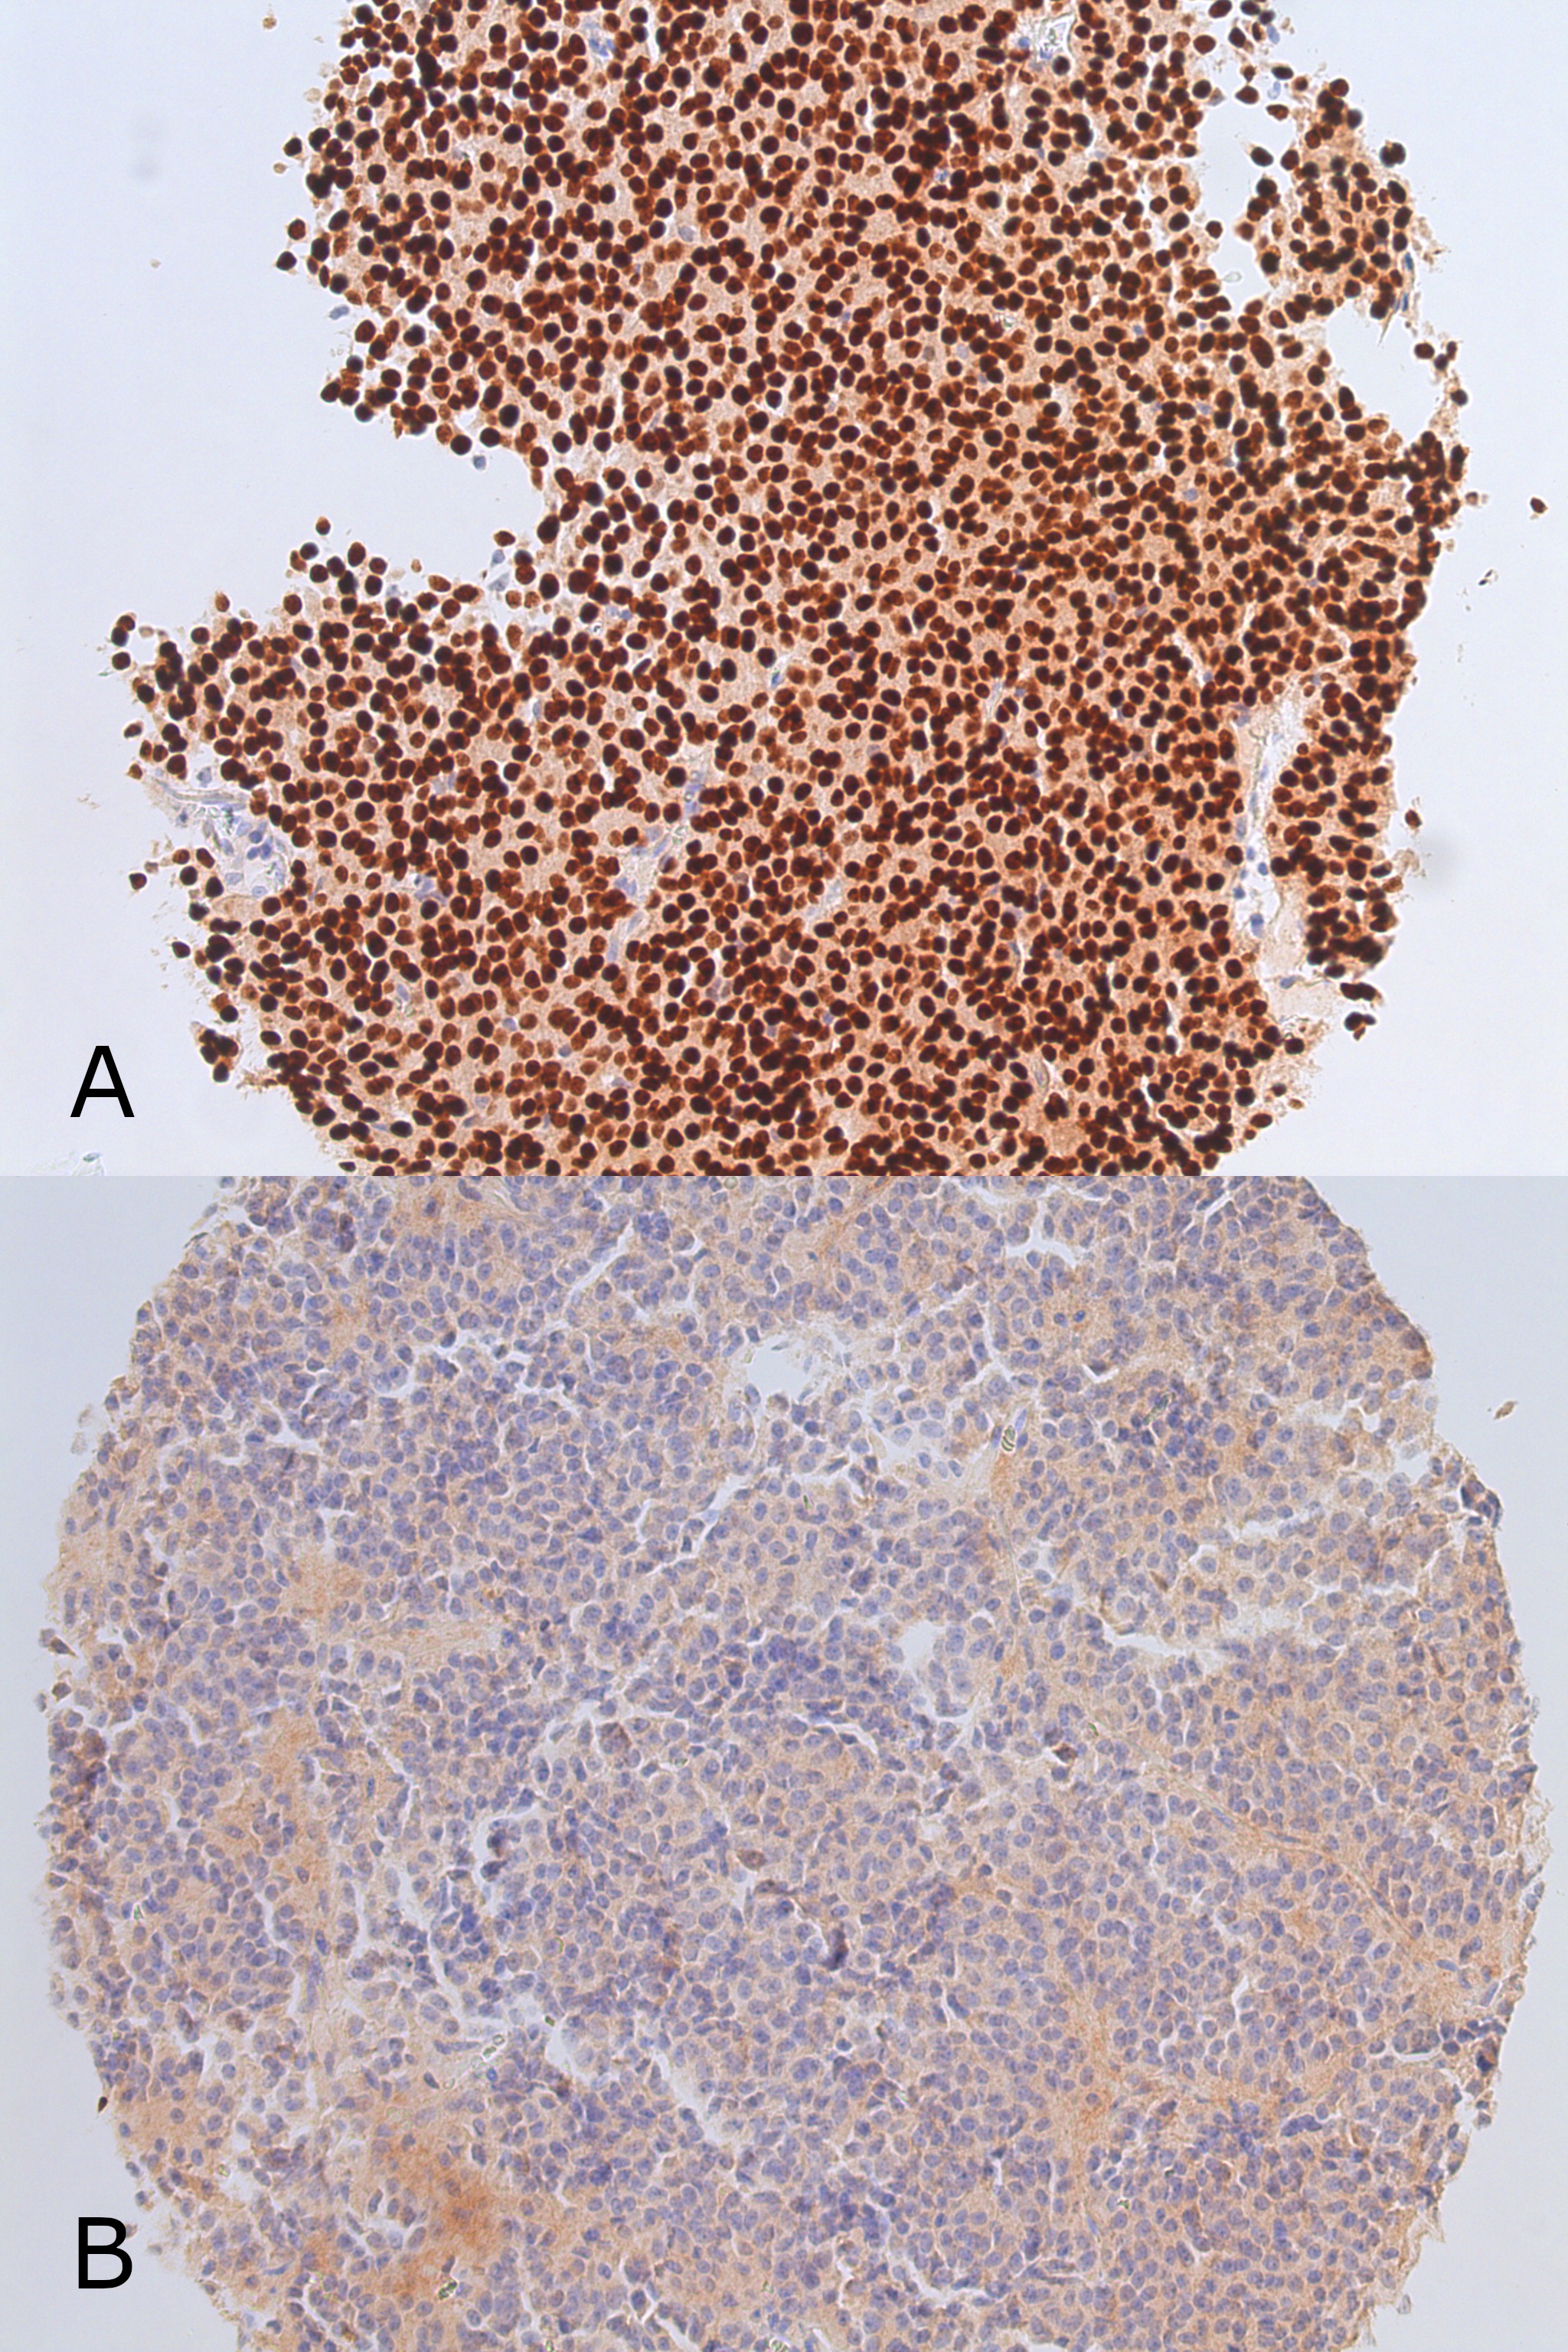
\includegraphics{_bookdown_files/pathologyImages/TpitIHC.jpg}
\caption{Tpit immunohistochemical stain. Figure A silent corticotroph. Figure B gonadotroph}
\end{figure}

Some of the subdirectories throw an error in building the book, so I settled on \texttt{\_bookdown\_files/pathologyImages} as the location.

Also, I note that the build does not generate the caption unless the reference is on it's own line.

Also note that some controls on image size are available. For instance, the same image can be displayed at 50\% size:

\begin{figure}
\hypertarget{id}{%
\centering
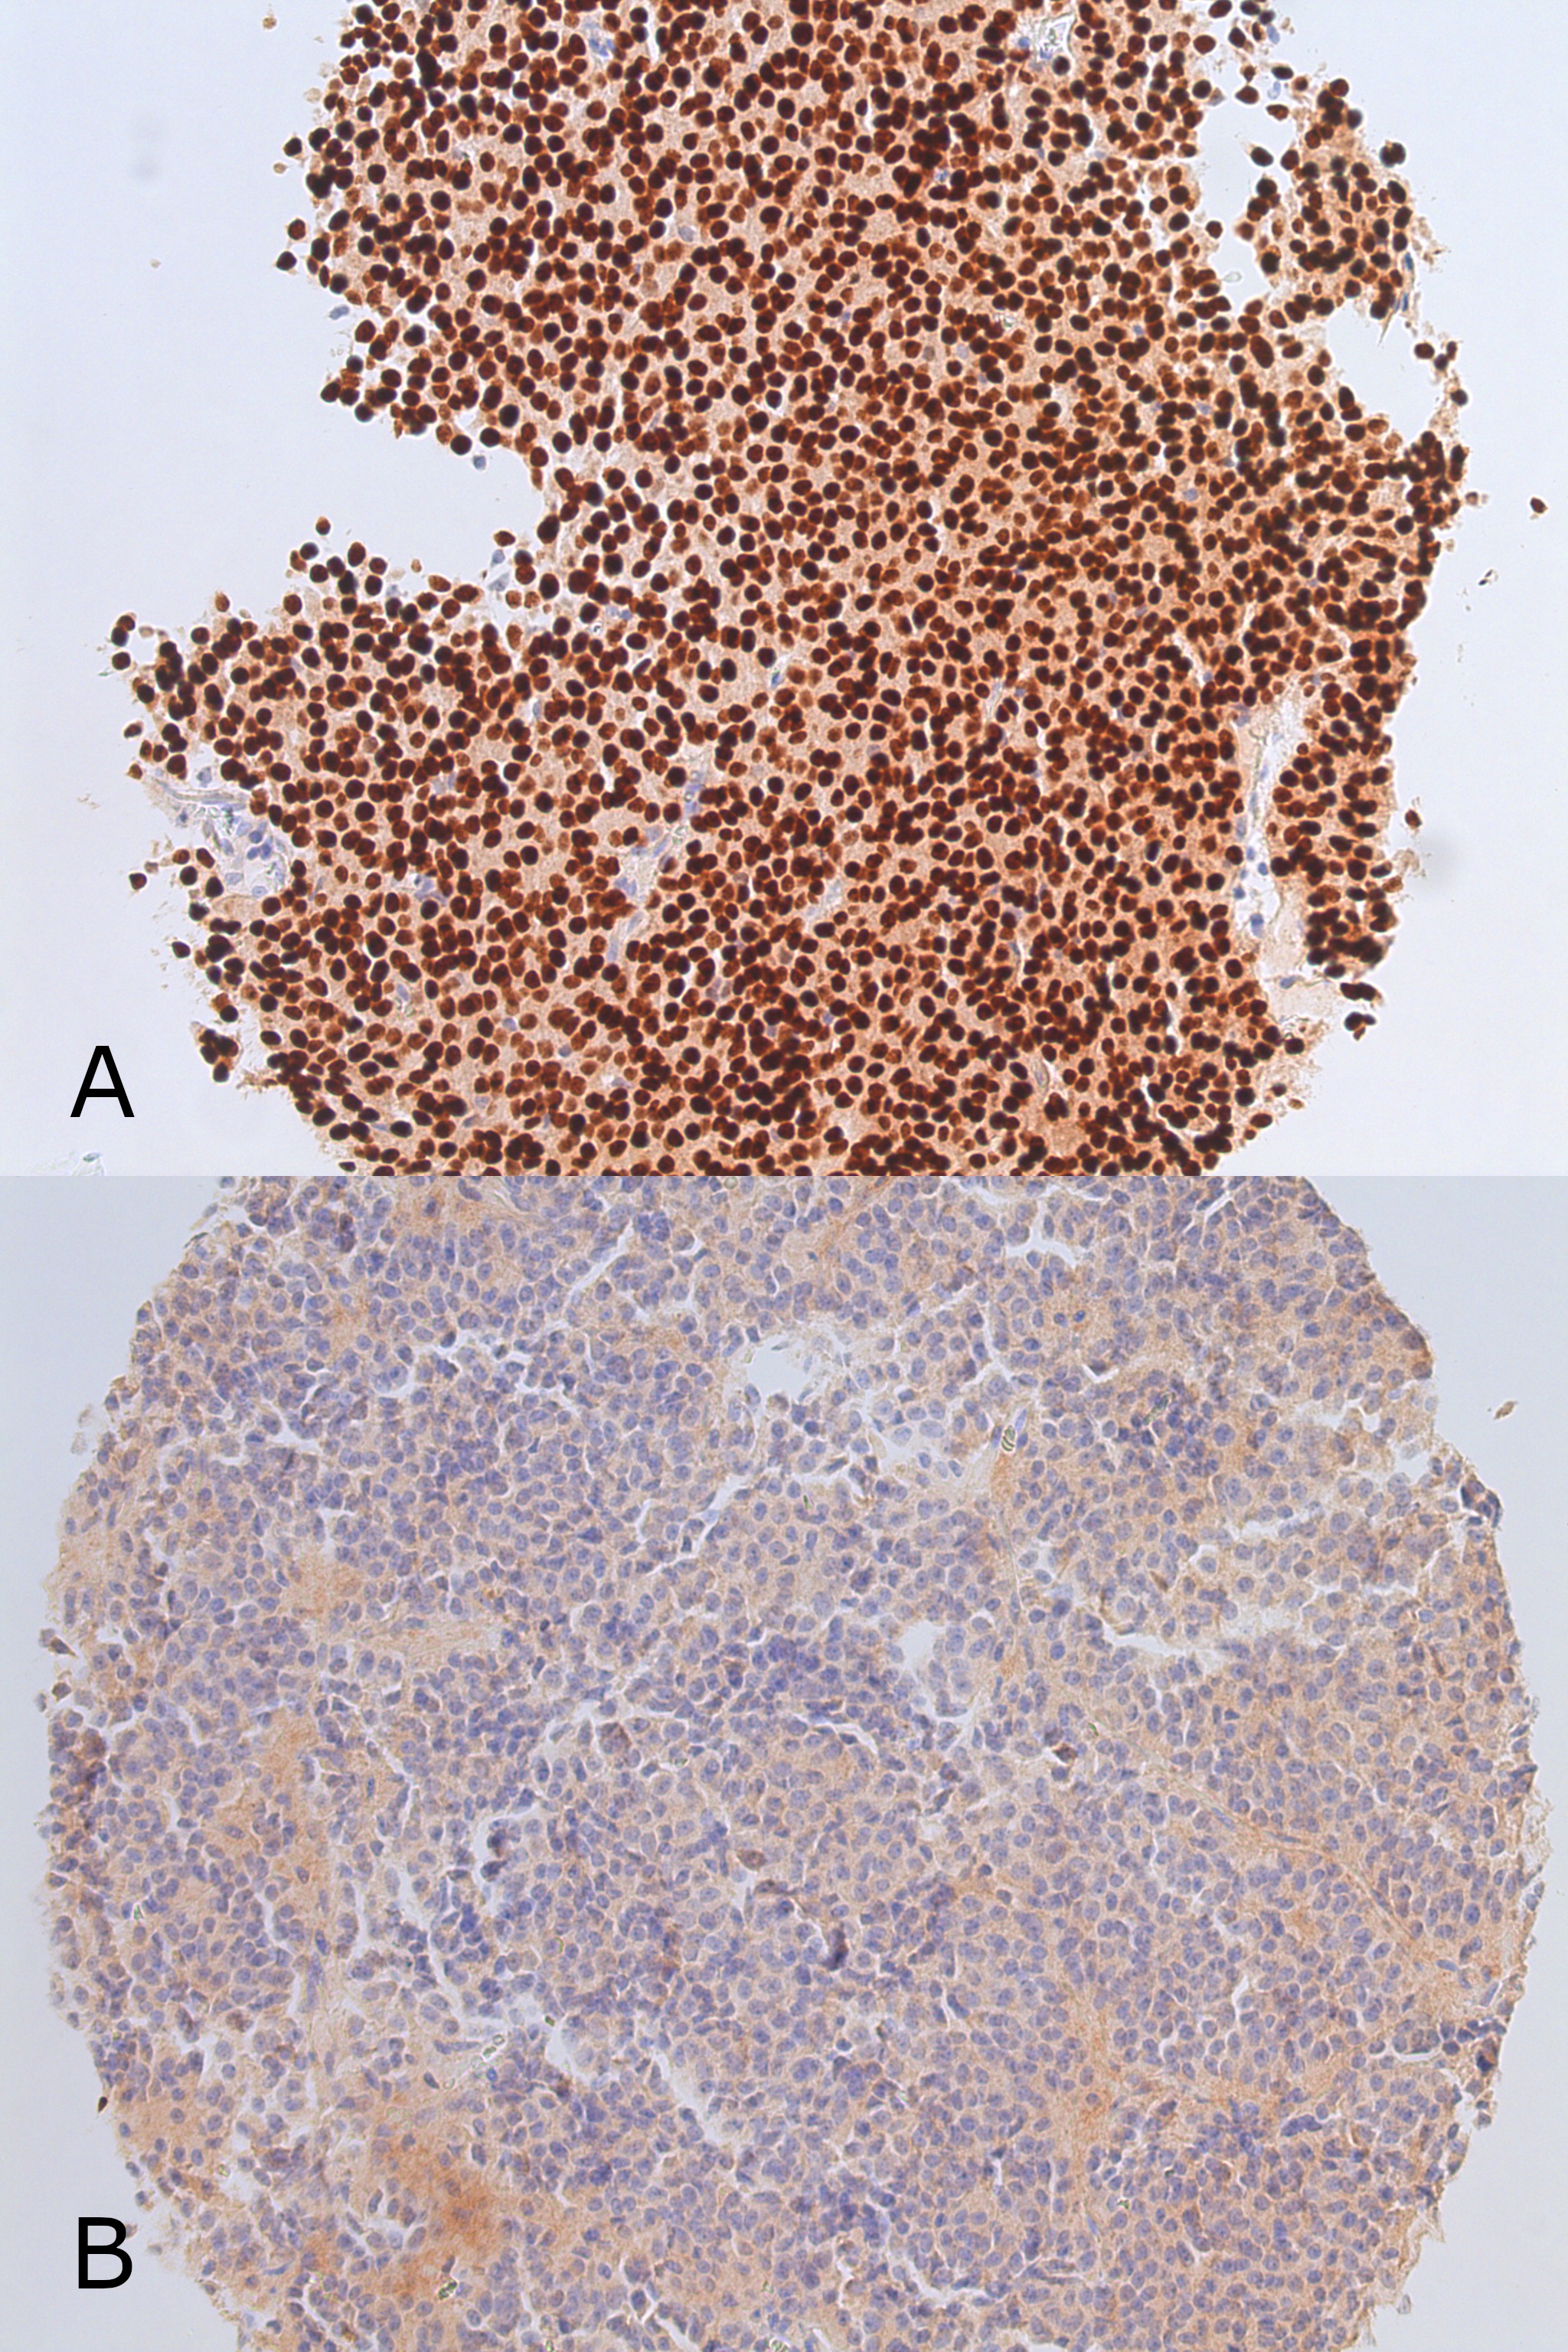
\includegraphics[width=0.5\textwidth,height=0.5\textheight]{_bookdown_files/pathologyImages/TpitIHC.jpg}
\caption{Tpit immunohistochemical stain. Figure A silent corticotroph. Figure B gonadotroph}\label{id}
}
\end{figure}

\hypertarget{referencing-citations}{%
\section{Referencing citations:}\label{referencing-citations}}

In order to insert citations, one needs a .bib file in the project. I've included one in this project as \texttt{book.bib}. The yml header in Chapter \ref{intro} needs to have a \(bibliography:\) and \(biblio-style:\) line added.

To insert a citation, use the \textbf{citr} Addin from RStudio. \textbf{bookdown}, for instance, is cited thusly \citep{R-bookdown}. Note that I need to figure out an adequate workflow of references. The convenience of Endnote in MS Word will not be available. Nonetheless, if I populate the book.bib and packages.bib files carefully, with .txt files generated in Endnote, I should be OK.

For instance, a recent dump of my Endnote library is in bookFromEndnote.txt. This can be opened in RStudio, and I can copy-and-paste references from the .txt file to my book.bib. For instance, if I have a breast paper that I want to cite here \citep{RN2750}, I'd copy-and-paste the reference from bookFromEndnot.text to book.bib.

Of note, Yihui Xie includes a nifty bit of code to automatically generate a bib database for R packages:

\begin{Shaded}
\begin{Highlighting}[]
\NormalTok{knitr}\OperatorTok{::}\KeywordTok{write_bib}\NormalTok{(}\KeywordTok{c}\NormalTok{(}\KeywordTok{.packages}\NormalTok{(), }\StringTok{'bookdown'}\NormalTok{, }\StringTok{'knitr'}\NormalTok{, }\StringTok{'rmarkdown'}\NormalTok{, }\StringTok{'tidyverse'}\NormalTok{, }\StringTok{'ComplexHeatmap'}\NormalTok{), }\StringTok{'packages.bib'}\NormalTok{)}
\end{Highlighting}
\end{Shaded}

References appear automatically at the end of a chapter.

\hypertarget{dataexploration}{%
\chapter{Data Exploration}\label{dataexploration}}

Data exploration is one of the most important aspects of data science and forms the cornerstone of my drills. Nonetheless, I have lots of room for improvement.

I like Hadely Wickham's writing and find his approach exceptionally clear. Therefore, I'll use the \textbf{tidyverse}.

\begin{Shaded}
\begin{Highlighting}[]
\KeywordTok{library}\NormalTok{(tidyverse)}
\end{Highlighting}
\end{Shaded}

\hypertarget{counting-things.-the-naming-of-parts.}{%
\section{Counting things. The naming of parts.}\label{counting-things.-the-naming-of-parts.}}

\begin{Shaded}
\begin{Highlighting}[]
\NormalTok{starwars }\OperatorTok\StringTok{ }
\StringTok{  }\KeywordTok{filter}\NormalTok{(}\OperatorTok{!}\KeywordTok{is.na}\NormalTok{(species)) }\OperatorTok\StringTok{ }
\StringTok{  }\KeywordTok{count}\NormalTok{(}\DataTypeTok{species =} \KeywordTok{fct_lump}\NormalTok{(species, }\DecValTok{5}\NormalTok{), }\DataTypeTok{sort =} \OtherTok{TRUE}\NormalTok{) }\OperatorTok\StringTok{ }
\StringTok{  }\KeywordTok{mutate}\NormalTok{(}\DataTypeTok{species =} \KeywordTok{fct_reorder}\NormalTok{(species, n)) }\OperatorTok\StringTok{ }
\StringTok{  }\KeywordTok{ggplot}\NormalTok{(}\KeywordTok{aes}\NormalTok{(species, n)) }\OperatorTok{+}\StringTok{ }
\StringTok{  }\KeywordTok{geom_col}\NormalTok{() }\OperatorTok{+}\StringTok{ }\KeywordTok{coord_flip}\NormalTok{()}
\end{Highlighting}
\end{Shaded}

\begin{figure}
\centering
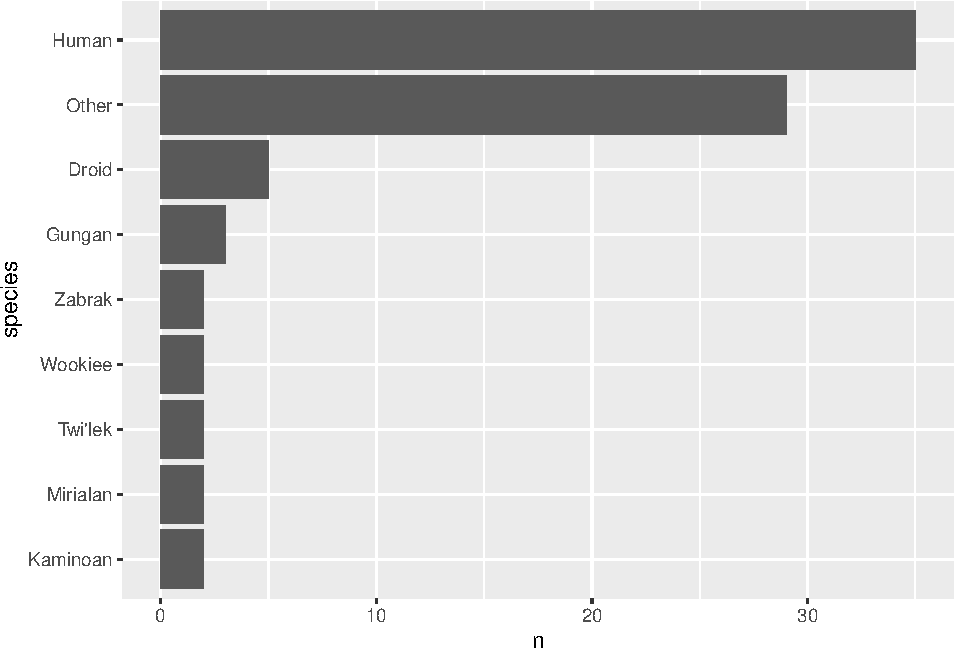
\includegraphics{test-book_files/figure-latex/starfig-1-1.pdf}
\caption{\label{fig:starfig-1}Starwars Figure 1}
\end{figure}

I like stacked bars for their economy, but it's easy to over do it. Supperimposing gender onto the columns seems easy\ldots{}

\begin{Shaded}
\begin{Highlighting}[]
\NormalTok{starwars }\OperatorTok\StringTok{ }
\StringTok{  }\KeywordTok{filter}\NormalTok{(}\OperatorTok{!}\KeywordTok{is.na}\NormalTok{(species)) }\OperatorTok\StringTok{ }
\StringTok{  }\KeywordTok{count}\NormalTok{(}\DataTypeTok{species =} \KeywordTok{fct_lump}\NormalTok{(species, }\DecValTok{5}\NormalTok{), }\DataTypeTok{gender =} \KeywordTok{fct_lump}\NormalTok{(gender, }\DecValTok{2}\NormalTok{), }\DataTypeTok{sort =} \OtherTok{TRUE}\NormalTok{) }\OperatorTok\StringTok{ }
\StringTok{  }\KeywordTok{mutate}\NormalTok{(}\DataTypeTok{species =} \KeywordTok{fct_reorder}\NormalTok{(species, n)) }\OperatorTok\StringTok{ }
\StringTok{  }\KeywordTok{ggplot}\NormalTok{(}\KeywordTok{aes}\NormalTok{(species, n, }\DataTypeTok{fill =}\NormalTok{ gender)) }\OperatorTok{+}\StringTok{ }
\StringTok{  }\KeywordTok{geom_col}\NormalTok{() }\OperatorTok{+}\StringTok{ }\KeywordTok{coord_flip}\NormalTok{()}
\end{Highlighting}
\end{Shaded}

\begin{verbatim}
## Warning: Factor `gender` contains implicit NA, consider using
## `forcats::fct_explicit_na`
\end{verbatim}

\begin{figure}
\centering
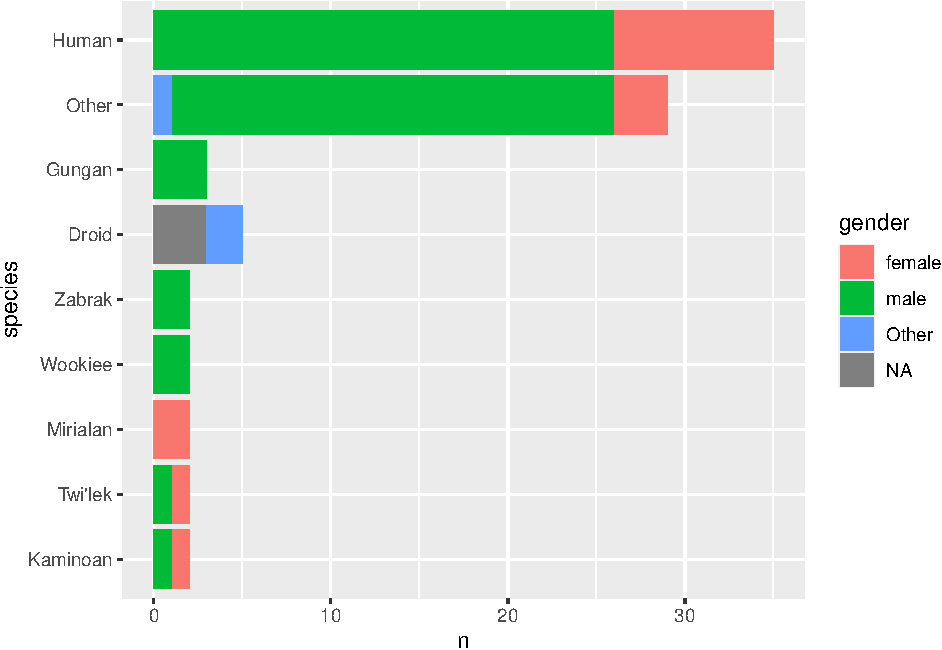
\includegraphics{test-book_files/figure-latex/starfig-2-1.pdf}
\caption{\label{fig:starfig-2}Starwars Figure 2}
\end{figure}

But note that I've got a problem: the Droids, which outnumber the Gungans, are now reordered to \emph{after} the Gungans. This happens because the \(n\) that we're counting comprises subcategories of species \emph{and} gender. Only three Gungan males exist (and no females), but that is enough to tie the Droid NA category. The Droid NA category come after the Gungan category, presumably because \emph{male} comes before \emph{NA}, or because NA comes last (more likely).

Exploring this, I see that I'm getting warning messages about the implicit NA's in gender. Note that the following renders a slightly different plot. I \emph{still} have not fixed the order of the species.

\begin{Shaded}
\begin{Highlighting}[]
\NormalTok{starwars }\OperatorTok\StringTok{ }
\StringTok{  }\KeywordTok{filter}\NormalTok{(}\OperatorTok{!}\KeywordTok{is.na}\NormalTok{(species)) }\OperatorTok\StringTok{ }
\StringTok{  }\KeywordTok{count}\NormalTok{(}\DataTypeTok{species =} \KeywordTok{fct_lump}\NormalTok{(species, }\DecValTok{5}\NormalTok{), }\DataTypeTok{gender =} \KeywordTok{fct_lump}\NormalTok{(gender, }\DecValTok{2}\NormalTok{), }\DataTypeTok{sort =} \OtherTok{TRUE}\NormalTok{) }\OperatorTok\StringTok{ }
\StringTok{  }\KeywordTok{mutate}\NormalTok{(}\DataTypeTok{gender =} \KeywordTok{fct_explicit_na}\NormalTok{(gender),}
         \DataTypeTok{species =} \KeywordTok{fct_reorder}\NormalTok{(species, n)) }\OperatorTok\StringTok{ }
\StringTok{  }\KeywordTok{ggplot}\NormalTok{(}\KeywordTok{aes}\NormalTok{(species, n, }\DataTypeTok{fill =}\NormalTok{ gender)) }\OperatorTok{+}\StringTok{ }
\StringTok{  }\KeywordTok{geom_col}\NormalTok{() }\OperatorTok{+}\StringTok{ }\KeywordTok{coord_flip}\NormalTok{()}
\end{Highlighting}
\end{Shaded}

\begin{verbatim}
## Warning: Factor `gender` contains implicit NA, consider using
## `forcats::fct_explicit_na`
\end{verbatim}

\begin{figure}
\centering
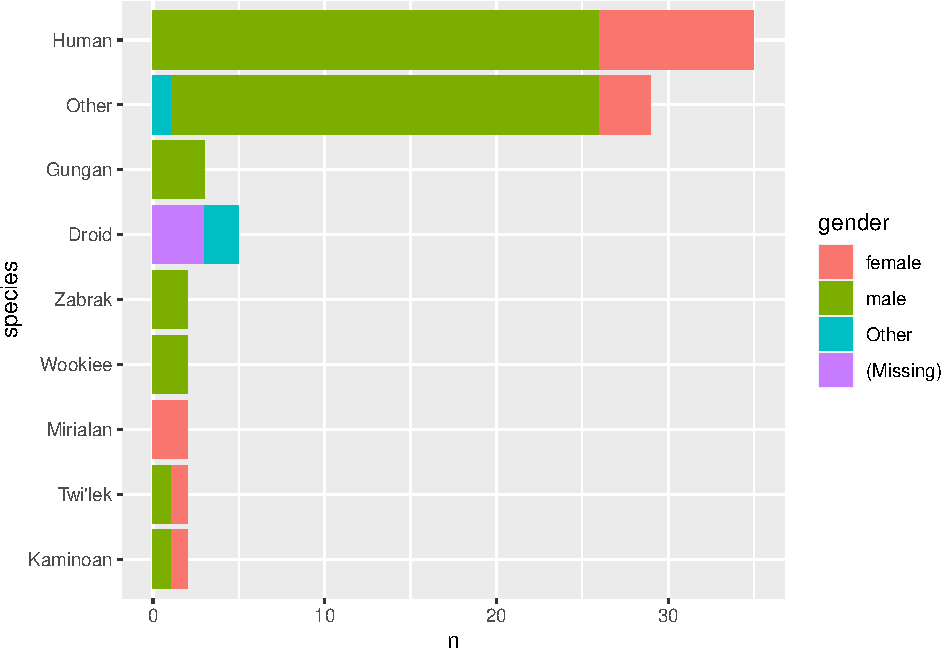
\includegraphics{test-book_files/figure-latex/starfig-3-1.pdf}
\caption{\label{fig:starfig-3}Starwars Figure 3}
\end{figure}

The trick here is to use \texttt{group\_by()} and \texttt{ungroup()} wisely.

\begin{Shaded}
\begin{Highlighting}[]
\NormalTok{starwars }\OperatorTok\StringTok{ }\KeywordTok{filter}\NormalTok{(}\OperatorTok{!}\KeywordTok{is.na}\NormalTok{(species)) }\OperatorTok\StringTok{ }
\StringTok{  }\KeywordTok{mutate}\NormalTok{(}\DataTypeTok{species =} \KeywordTok{fct_lump}\NormalTok{(species, }\DecValTok{5}\NormalTok{)) }\OperatorTok\StringTok{ }
\StringTok{  }\KeywordTok{group_by}\NormalTok{(species) }\OperatorTok\StringTok{ }
\StringTok{  }\KeywordTok{mutate}\NormalTok{(}\DataTypeTok{typeCount =} \KeywordTok{n}\NormalTok{()) }\OperatorTok\StringTok{ }
\StringTok{  }\KeywordTok{ungroup}\NormalTok{() }\OperatorTok\StringTok{ }
\StringTok{  }\KeywordTok{mutate}\NormalTok{(}\DataTypeTok{species =} \KeywordTok{fct_reorder}\NormalTok{(species, typeCount)) }\OperatorTok\StringTok{ }
\StringTok{  }\KeywordTok{ggplot}\NormalTok{()}\OperatorTok{+}
\StringTok{  }\KeywordTok{geom_bar}\NormalTok{(}\KeywordTok{aes}\NormalTok{(species, }\DataTypeTok{fill =}\NormalTok{ gender))}\OperatorTok{+}
\StringTok{  }\KeywordTok{coord_flip}\NormalTok{()}
\end{Highlighting}
\end{Shaded}

\begin{figure}
\centering
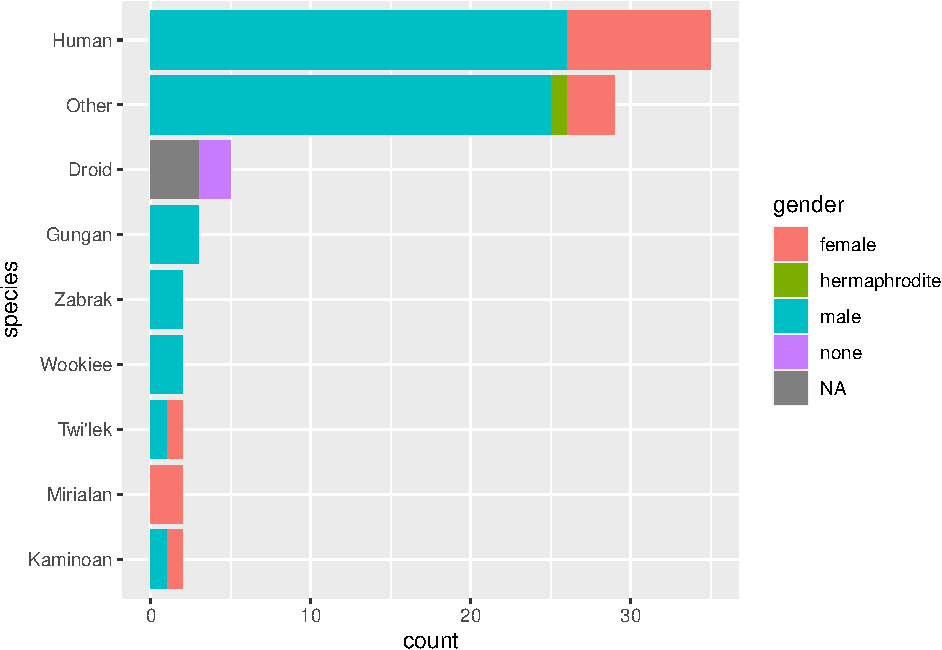
\includegraphics{test-book_files/figure-latex/starfig-4-1.pdf}
\caption{\label{fig:starfig-4}Starwars Figure 4}
\end{figure}

As opposed to using \texttt{count()}, which progressively narrows the information available to be used, by using \texttt{group\_by()}/\texttt{mutate()}/\texttt{ungroup()} with \texttt{geom\_bar()} we have all of the variables still available for plotting.

\hypertarget{summarize-is-another-very-useful-function}{%
\section{Summarize is another very useful function:}\label{summarize-is-another-very-useful-function}}

\begin{Shaded}
\begin{Highlighting}[]
\NormalTok{starwars }\OperatorTok\StringTok{ }
\StringTok{  }\KeywordTok{filter}\NormalTok{(}\OperatorTok{!}\NormalTok{(}\KeywordTok{is.na}\NormalTok{(species))) }\OperatorTok\StringTok{ }
\StringTok{  }\KeywordTok{group_by}\NormalTok{(species) }\OperatorTok\StringTok{ }
\StringTok{  }\KeywordTok{summarize}\NormalTok{(}\DataTypeTok{n=}\KeywordTok{n}\NormalTok{(), }\DataTypeTok{mean =} \KeywordTok{mean}\NormalTok{(height, }\DataTypeTok{na.rm =} \OtherTok{TRUE}\NormalTok{)) }\OperatorTok\StringTok{ }
\StringTok{  }\KeywordTok{arrange}\NormalTok{(}\KeywordTok{desc}\NormalTok{(n))}
\end{Highlighting}
\end{Shaded}

\begin{verbatim}
## # A tibble: 37 x 3
##    species      n  mean
##    <chr>    <int> <dbl>
##  1 Human       35  177.
##  2 Droid        5  140 
##  3 Gungan       3  209.
##  4 Kaminoan     2  221 
##  5 Mirialan     2  168 
##  6 Twi'lek      2  179 
##  7 Wookiee      2  231 
##  8 Zabrak       2  173 
##  9 Aleena       1   79 
## 10 Besalisk     1  198 
## # ... with 27 more rows
\end{verbatim}

\hypertarget{sampling}{%
\chapter{Sampling}\label{sampling}}

\hypertarget{think-about-throwing-a-bunch-of-dice.}{%
\section{Think about throwing a bunch of dice.}\label{think-about-throwing-a-bunch-of-dice.}}

\begin{Shaded}
\begin{Highlighting}[]
\KeywordTok{sample}\NormalTok{(}\DecValTok{1}\OperatorTok{:}\DecValTok{6}\NormalTok{, }\DataTypeTok{size=}\DecValTok{100}\NormalTok{, }\DataTypeTok{replace=}\OtherTok{TRUE}\NormalTok{) }
\end{Highlighting}
\end{Shaded}

\begin{verbatim}
##   [1] 4 3 6 3 4 2 1 4 1 4 4 3 4 2 2 1 3 3 3 2 6 4 4 3 3 4 1 5 3 6 3 1 1 2 2 5 2
##  [38] 2 6 3 5 3 5 3 4 6 4 3 2 3 2 6 1 5 6 1 4 4 4 2 1 5 1 6 3 1 5 2 6 1 2 3 6 3
##  [75] 1 4 5 5 4 6 6 4 5 2 6 2 6 6 1 6 2 2 3 6 4 2 6 4 6 6
\end{verbatim}

\begin{Shaded}
\begin{Highlighting}[]
\KeywordTok{sample}\NormalTok{(}\DecValTok{1}\OperatorTok{:}\DecValTok{6}\NormalTok{, }\DataTypeTok{size=}\DecValTok{100}\NormalTok{, }\DataTypeTok{replace=}\OtherTok{TRUE}\NormalTok{) }\OperatorTok\StringTok{ }\KeywordTok{table}\NormalTok{()}
\end{Highlighting}
\end{Shaded}

\begin{verbatim}
## .
##  1  2  3  4  5  6 
## 22 18 17 14 18 11
\end{verbatim}

\begin{Shaded}
\begin{Highlighting}[]
\KeywordTok{sample}\NormalTok{(}\DecValTok{1}\OperatorTok{:}\DecValTok{6}\NormalTok{, }\DataTypeTok{size=}\DecValTok{100}\NormalTok{, }\DataTypeTok{replace=}\OtherTok{TRUE}\NormalTok{) }\OperatorTok\StringTok{ }\KeywordTok{table}\NormalTok{() }\OperatorTok\StringTok{ }\KeywordTok{prop.table}\NormalTok{()}
\end{Highlighting}
\end{Shaded}

\begin{verbatim}
## .
##    1    2    3    4    5    6 
## 0.23 0.15 0.12 0.18 0.21 0.11
\end{verbatim}

\hypertarget{a-keen-way-to-divide-up-a-dataset-into-testing-and-training-components.}{%
\section{A keen way to divide up a dataset into testing and training components.}\label{a-keen-way-to-divide-up-a-dataset-into-testing-and-training-components.}}

\begin{Shaded}
\begin{Highlighting}[]
\NormalTok{x <-}\StringTok{ }\DecValTok{1}\OperatorTok{:}\DecValTok{10}
\NormalTok{y <-}\StringTok{ }\DecValTok{11}\OperatorTok{:}\DecValTok{30}

\NormalTok{df <-}\StringTok{ }\KeywordTok{data.frame}\NormalTok{(x,y)}
\NormalTok{df}
\end{Highlighting}
\end{Shaded}

\begin{verbatim}
##     x  y
## 1   1 11
## 2   2 12
## 3   3 13
## 4   4 14
## 5   5 15
## 6   6 16
## 7   7 17
## 8   8 18
## 9   9 19
## 10 10 20
## 11  1 21
## 12  2 22
## 13  3 23
## 14  4 24
## 15  5 25
## 16  6 26
## 17  7 27
## 18  8 28
## 19  9 29
## 20 10 30
\end{verbatim}

\begin{Shaded}
\begin{Highlighting}[]
\KeywordTok{set.seed}\NormalTok{(}\DecValTok{0}\NormalTok{)}
\NormalTok{train_indexes =}\StringTok{ }\KeywordTok{sample}\NormalTok{(}\DecValTok{1}\OperatorTok{:}\KeywordTok{nrow}\NormalTok{(df), }\FloatTok{.7} \OperatorTok{*}\StringTok{ }\KeywordTok{nrow}\NormalTok{(df))}

\NormalTok{train_set <-}\StringTok{ }\NormalTok{df[train_indexes,]}
\NormalTok{test_set <-}\StringTok{ }\NormalTok{df[}\OperatorTok{-}\NormalTok{train_indexes,]}

\NormalTok{train_set}
\end{Highlighting}
\end{Shaded}

\begin{verbatim}
##    x  y
## 14 4 24
## 4  4 14
## 7  7 17
## 1  1 11
## 2  2 12
## 13 3 23
## 18 8 28
## 11 1 21
## 16 6 26
## 15 5 25
## 3  3 13
## 17 7 27
## 5  5 15
## 8  8 18
\end{verbatim}

\begin{Shaded}
\begin{Highlighting}[]
\NormalTok{test_set}
\end{Highlighting}
\end{Shaded}

\begin{verbatim}
##     x  y
## 6   6 16
## 9   9 19
## 10 10 20
## 12  2 22
## 19  9 29
## 20 10 30
\end{verbatim}

\hypertarget{factorpractice}{%
\chapter{Factor Practice}\label{factorpractice}}

\begin{Shaded}
\begin{Highlighting}[]
\NormalTok{cups <-}\StringTok{ }\KeywordTok{c}\NormalTok{(}\StringTok{"small"}\NormalTok{, }\StringTok{"medium"}\NormalTok{, }\StringTok{"large"}\NormalTok{)}
\NormalTok{manyCups <-}\StringTok{ }\KeywordTok{sample}\NormalTok{(cups, }\DataTypeTok{size =} \DecValTok{100}\NormalTok{, }\DataTypeTok{replace =} \OtherTok{TRUE}\NormalTok{)}
\NormalTok{sizesCups <-}\StringTok{ }\KeywordTok{factor}\NormalTok{(manyCups, }\DataTypeTok{levels =} \KeywordTok{c}\NormalTok{(}\StringTok{"small"}\NormalTok{, }\StringTok{"medium"}\NormalTok{, }\StringTok{"large"}\NormalTok{))}
\NormalTok{sizesCups}
\end{Highlighting}
\end{Shaded}

\begin{verbatim}
##   [1] medium medium medium medium large  small  large  small  small  small 
##  [11] small  medium small  small  medium medium medium small  large  small 
##  [21] large  medium medium medium medium large  medium small  large  medium
##  [31] small  small  large  medium medium large  large  medium medium medium
##  [41] medium small  medium medium medium medium small  large  large  medium
##  [51] large  large  medium large  large  small  small  small  small  large 
##  [61] medium large  small  small  medium small  small  small  small  large 
##  [71] medium small  small  large  large  large  medium medium medium large 
##  [81] medium medium large  large  large  small  medium medium small  large 
##  [91] large  medium large  medium small  medium small  large  large  small 
## Levels: small medium large
\end{verbatim}

\hypertarget{crossingtrial}{%
\chapter{Crossing Trial}\label{crossingtrial}}

From David Robinson birthday paradox Rblogger at \url{https://www.r-bloggers.com/the-birthday-paradox-puzzle-tidy-simulation-in-r/}

\begin{Shaded}
\begin{Highlighting}[]
\NormalTok{summarized <-}\StringTok{ }\KeywordTok{crossing}\NormalTok{(}\DataTypeTok{people =} \KeywordTok{seq}\NormalTok{(}\DecValTok{2}\NormalTok{, }\DecValTok{50}\NormalTok{, }\DecValTok{2}\NormalTok{),}
                       \DataTypeTok{trial =} \DecValTok{1}\OperatorTok{:}\DecValTok{100}\NormalTok{) }\OperatorTok
\StringTok{  }\KeywordTok{mutate}\NormalTok{(}\DataTypeTok{birthday =} \KeywordTok{map}\NormalTok{(people, }\OperatorTok{~}\StringTok{ }\KeywordTok{sample}\NormalTok{(}\DecValTok{365}\NormalTok{, .x, }\DataTypeTok{replace =} \OtherTok{TRUE}\NormalTok{)),}
         \DataTypeTok{multiple =} \KeywordTok{map_lgl}\NormalTok{(birthday, }\OperatorTok{~}\StringTok{ }\KeywordTok{any}\NormalTok{(}\KeywordTok{duplicated}\NormalTok{(.x)))) }\OperatorTok
\StringTok{  }\KeywordTok{group_by}\NormalTok{(people) }\OperatorTok
\StringTok{  }\KeywordTok{summarize}\NormalTok{(}\DataTypeTok{chance =} \KeywordTok{mean}\NormalTok{(multiple))}

\KeywordTok{ggplot}\NormalTok{(summarized, }\KeywordTok{aes}\NormalTok{(people, chance)) }\OperatorTok{+}
\StringTok{  }\KeywordTok{geom_line}\NormalTok{() }\OperatorTok{+}
\StringTok{  }\KeywordTok{scale_y_continuous}\NormalTok{(}\DataTypeTok{labels =}\NormalTok{ scales}\OperatorTok{::}\KeywordTok{percent_format}\NormalTok{()) }\OperatorTok{+}
\StringTok{  }\KeywordTok{labs}\NormalTok{(}\DataTypeTok{y =} \StringTok{"Probability two have the same birthday"}\NormalTok{)}
\end{Highlighting}
\end{Shaded}

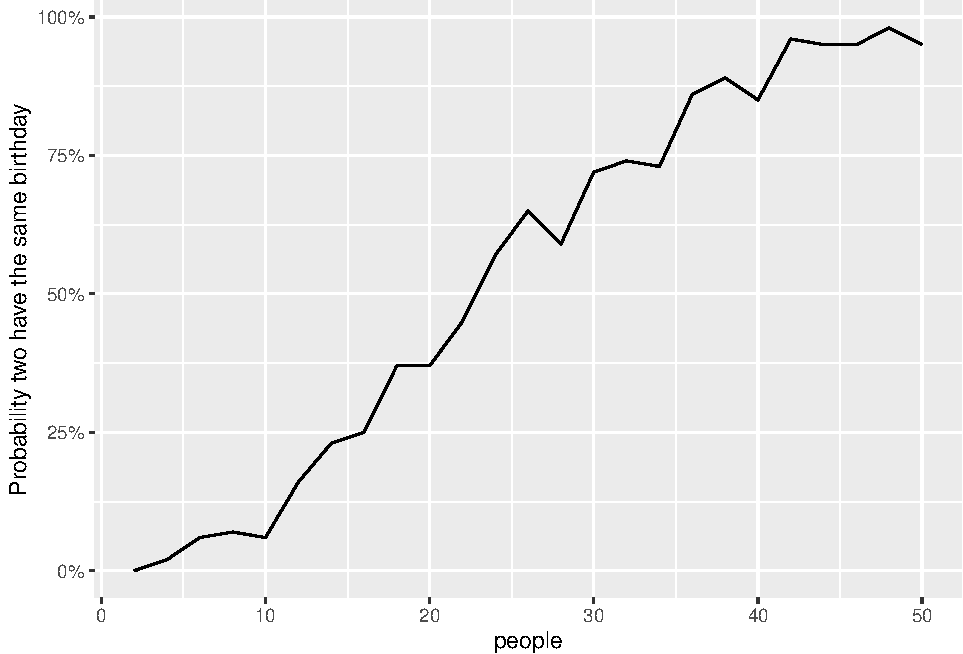
\includegraphics{test-book_files/figure-latex/unnamed-chunk-7-1.pdf}

\begin{Shaded}
\begin{Highlighting}[]
\CommentTok{# Checking the work with pbirthday function}
\NormalTok{summarized }\OperatorTok\StringTok{ }
\StringTok{  }\KeywordTok{mutate}\NormalTok{(}\DataTypeTok{exact =} \KeywordTok{map_dbl}\NormalTok{(people, pbirthday)) }\OperatorTok\StringTok{ }
\StringTok{  }\KeywordTok{ggplot}\NormalTok{(}\KeywordTok{aes}\NormalTok{(people, chance)) }\OperatorTok{+}
\StringTok{  }\KeywordTok{geom_line}\NormalTok{() }\OperatorTok{+}
\StringTok{  }\KeywordTok{geom_line}\NormalTok{(}\KeywordTok{aes}\NormalTok{(}\DataTypeTok{y =}\NormalTok{ exact), }\DataTypeTok{lty =} \DecValTok{2}\NormalTok{, }\DataTypeTok{color =} \StringTok{"blue"}\NormalTok{) }\OperatorTok{+}
\StringTok{  }\KeywordTok{scale_y_continuous}\NormalTok{(}\DataTypeTok{labels =}\NormalTok{ scales}\OperatorTok{::}\KeywordTok{percent_format}\NormalTok{()) }\OperatorTok{+}
\StringTok{  }\KeywordTok{labs}\NormalTok{(}\DataTypeTok{y =} \StringTok{"Probability two have the same birthday"}\NormalTok{)}
\end{Highlighting}
\end{Shaded}

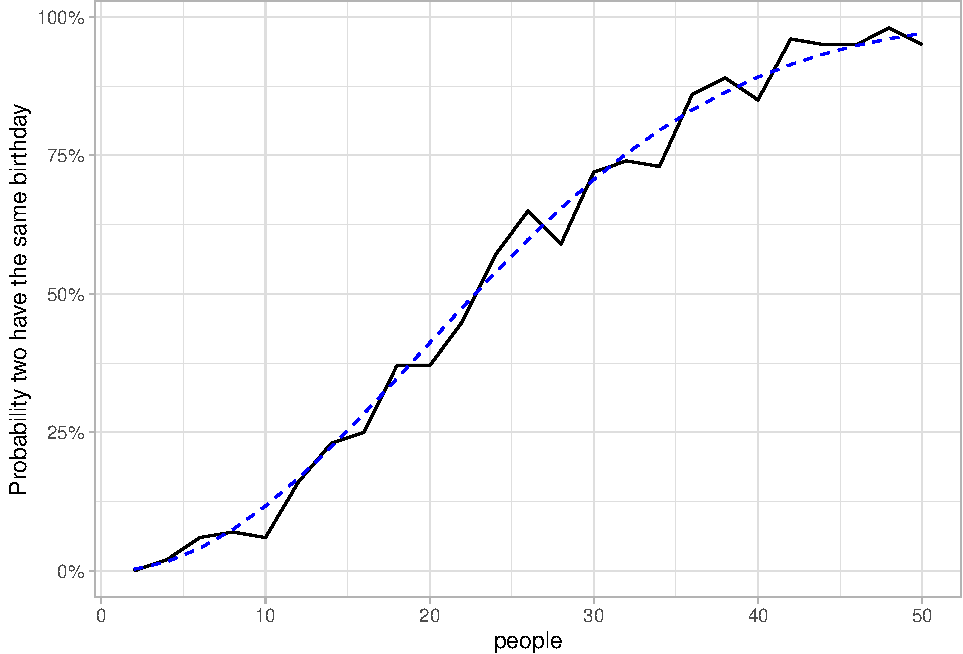
\includegraphics{test-book_files/figure-latex/unnamed-chunk-7-2.pdf}

\hypertarget{changenames}{%
\chapter{By Any Other Name}\label{changenames}}

This deceptively simple-seeming idea gets complex quickly. The following YouTube was a nice description of the process: \url{https://www.youtube.com/watch?v=Okc0IL5uTnA}

\begin{Shaded}
\begin{Highlighting}[]
\NormalTok{my.data <-}\StringTok{ }\KeywordTok{data.frame}\NormalTok{(}\DataTypeTok{colOne=}\DecValTok{1}\OperatorTok{:}\DecValTok{3}\NormalTok{, }\DataTypeTok{column2=}\DecValTok{4}\OperatorTok{:}\DecValTok{6}\NormalTok{, }\DataTypeTok{column_3=}\DecValTok{7}\OperatorTok{:}\DecValTok{9}\NormalTok{)}
\KeywordTok{rownames}\NormalTok{(my.data) <-}\StringTok{ }\KeywordTok{c}\NormalTok{(}\StringTok{"ant"}\NormalTok{, }\StringTok{"bee"}\NormalTok{, }\StringTok{"cat"}\NormalTok{)}
\KeywordTok{names}\NormalTok{(my.data)}
\end{Highlighting}
\end{Shaded}

\begin{verbatim}
## [1] "colOne"   "column2"  "column_3"
\end{verbatim}

\begin{Shaded}
\begin{Highlighting}[]
\KeywordTok{colnames}\NormalTok{(my.data)}
\end{Highlighting}
\end{Shaded}

\begin{verbatim}
## [1] "colOne"   "column2"  "column_3"
\end{verbatim}

\begin{Shaded}
\begin{Highlighting}[]
\CommentTok{#make some changes}
\KeywordTok{names}\NormalTok{(my.data) <-}\StringTok{ }\KeywordTok{c}\NormalTok{(}\StringTok{"col_1"}\NormalTok{, }\StringTok{"col_2"}\NormalTok{, }\StringTok{"col_3"}\NormalTok{)}
\NormalTok{my.data}
\end{Highlighting}
\end{Shaded}

\begin{verbatim}
##     col_1 col_2 col_3
## ant     1     4     7
## bee     2     5     8
## cat     3     6     9
\end{verbatim}

\begin{Shaded}
\begin{Highlighting}[]
\KeywordTok{names}\NormalTok{(my.data)[}\DecValTok{3}\NormalTok{] <-}\StringTok{ "col.3"}
\NormalTok{my.data}
\end{Highlighting}
\end{Shaded}

\begin{verbatim}
##     col_1 col_2 col.3
## ant     1     4     7
## bee     2     5     8
## cat     3     6     9
\end{verbatim}

\begin{Shaded}
\begin{Highlighting}[]
\KeywordTok{names}\NormalTok{(my.data)[}\KeywordTok{names}\NormalTok{(my.data)}\OperatorTok{==}\StringTok{"col_2"}\NormalTok{]}
\end{Highlighting}
\end{Shaded}

\begin{verbatim}
## [1] "col_2"
\end{verbatim}

\begin{Shaded}
\begin{Highlighting}[]
\NormalTok{my.data[}\StringTok{"col_2"}\NormalTok{]}
\end{Highlighting}
\end{Shaded}

\begin{verbatim}
##     col_2
## ant     4
## bee     5
## cat     6
\end{verbatim}

\begin{Shaded}
\begin{Highlighting}[]
\NormalTok{my.data}\OperatorTok{$}\NormalTok{col_}\DecValTok{2}
\end{Highlighting}
\end{Shaded}

\begin{verbatim}
## [1] 4 5 6
\end{verbatim}

\begin{Shaded}
\begin{Highlighting}[]
\NormalTok{my.data[,}\DecValTok{2}\NormalTok{]}
\end{Highlighting}
\end{Shaded}

\begin{verbatim}
## [1] 4 5 6
\end{verbatim}

\begin{Shaded}
\begin{Highlighting}[]
\KeywordTok{names}\NormalTok{(my.data)[}\KeywordTok{names}\NormalTok{(my.data)}\OperatorTok{==}\StringTok{"col_2"}\NormalTok{] <-}\StringTok{ "col.2"}
\NormalTok{my.data}
\end{Highlighting}
\end{Shaded}

\begin{verbatim}
##     col_1 col.2 col.3
## ant     1     4     7
## bee     2     5     8
## cat     3     6     9
\end{verbatim}

\begin{Shaded}
\begin{Highlighting}[]
\KeywordTok{names}\NormalTok{(my.data) <-}\StringTok{ }\KeywordTok{gsub}\NormalTok{(}\StringTok{"_"}\NormalTok{, }\StringTok{"."}\NormalTok{, }\KeywordTok{names}\NormalTok{(my.data))}
\NormalTok{my.data}
\end{Highlighting}
\end{Shaded}

\begin{verbatim}
##     col.1 col.2 col.3
## ant     1     4     7
## bee     2     5     8
## cat     3     6     9
\end{verbatim}

\begin{Shaded}
\begin{Highlighting}[]
\KeywordTok{rownames}\NormalTok{(my.data)}
\end{Highlighting}
\end{Shaded}

\begin{verbatim}
## [1] "ant" "bee" "cat"
\end{verbatim}

\begin{Shaded}
\begin{Highlighting}[]
\NormalTok{my.data}\OperatorTok{$}\NormalTok{species <-}\StringTok{ }\KeywordTok{rownames}\NormalTok{(my.data)}
\NormalTok{my.data}
\end{Highlighting}
\end{Shaded}

\begin{verbatim}
##     col.1 col.2 col.3 species
## ant     1     4     7     ant
## bee     2     5     8     bee
## cat     3     6     9     cat
\end{verbatim}

\begin{Shaded}
\begin{Highlighting}[]
\KeywordTok{rownames}\NormalTok{(my.data) <-}\StringTok{ }\OtherTok{NULL}
\NormalTok{my.data}
\end{Highlighting}
\end{Shaded}

\begin{verbatim}
##   col.1 col.2 col.3 species
## 1     1     4     7     ant
## 2     2     5     8     bee
## 3     3     6     9     cat
\end{verbatim}

\begin{Shaded}
\begin{Highlighting}[]
\KeywordTok{colnames}\NormalTok{(my.data) <-}\StringTok{ }\KeywordTok{c}\NormalTok{(}\StringTok{"good"}\NormalTok{, }\StringTok{"better"}\NormalTok{, }\StringTok{"best"}\NormalTok{, }\StringTok{"species"}\NormalTok{)}
\NormalTok{my.data}
\end{Highlighting}
\end{Shaded}

\begin{verbatim}
##   good better best species
## 1    1      4    7     ant
## 2    2      5    8     bee
## 3    3      6    9     cat
\end{verbatim}

\begin{Shaded}
\begin{Highlighting}[]
\NormalTok{keep <-}\StringTok{ }\DecValTok{2}\OperatorTok{:}\KeywordTok{ncol}\NormalTok{(my.data)}
\NormalTok{my.data[,keep]}
\end{Highlighting}
\end{Shaded}

\begin{verbatim}
##   better best species
## 1      4    7     ant
## 2      5    8     bee
## 3      6    9     cat
\end{verbatim}

\hypertarget{correlation}{%
\chapter{Correlation Plots}\label{correlation}}

\begin{Shaded}
\begin{Highlighting}[]
\KeywordTok{head}\NormalTok{(iris)}
\end{Highlighting}
\end{Shaded}

\begin{verbatim}
##   Sepal.Length Sepal.Width Petal.Length Petal.Width Species
## 1          5.1         3.5          1.4         0.2  setosa
## 2          4.9         3.0          1.4         0.2  setosa
## 3          4.7         3.2          1.3         0.2  setosa
## 4          4.6         3.1          1.5         0.2  setosa
## 5          5.0         3.6          1.4         0.2  setosa
## 6          5.4         3.9          1.7         0.4  setosa
\end{verbatim}

\begin{Shaded}
\begin{Highlighting}[]
\NormalTok{iris }\OperatorTok\StringTok{ }\KeywordTok{select}\NormalTok{(}\OperatorTok{-}\NormalTok{Species) }\OperatorTok\StringTok{ }\KeywordTok{cor}\NormalTok{()}
\end{Highlighting}
\end{Shaded}

\begin{verbatim}
##              Sepal.Length Sepal.Width Petal.Length Petal.Width
## Sepal.Length    1.0000000  -0.1175698    0.8717538   0.8179411
## Sepal.Width    -0.1175698   1.0000000   -0.4284401  -0.3661259
## Petal.Length    0.8717538  -0.4284401    1.0000000   0.9628654
## Petal.Width     0.8179411  -0.3661259    0.9628654   1.0000000
\end{verbatim}

\begin{Shaded}
\begin{Highlighting}[]
\NormalTok{M <-}\StringTok{ }\NormalTok{iris }\OperatorTok\StringTok{ }\KeywordTok{select}\NormalTok{(}\OperatorTok{-}\NormalTok{Species) }\OperatorTok\StringTok{ }\KeywordTok{cor}\NormalTok{(}\DataTypeTok{method =} \StringTok{"kendall"}\NormalTok{)}
\end{Highlighting}
\end{Shaded}

\begin{Shaded}
\begin{Highlighting}[]
\NormalTok{corrplot}\OperatorTok{::}\KeywordTok{corrplot}\NormalTok{(M)}
\end{Highlighting}
\end{Shaded}

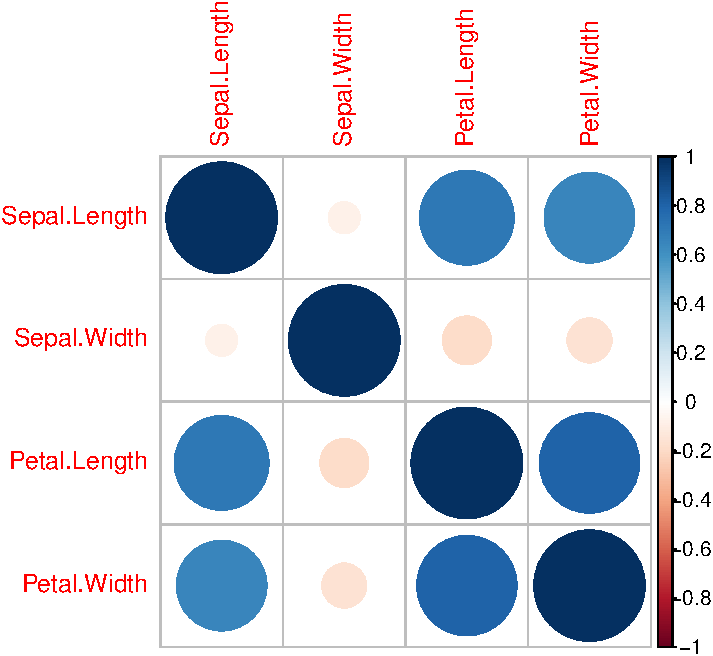
\includegraphics{test-book_files/figure-latex/unnamed-chunk-10-1.pdf}

\begin{Shaded}
\begin{Highlighting}[]
\NormalTok{corrplot}\OperatorTok{::}\KeywordTok{corrplot}\NormalTok{(M, }\DataTypeTok{method =} \StringTok{"color"}\NormalTok{)}
\end{Highlighting}
\end{Shaded}

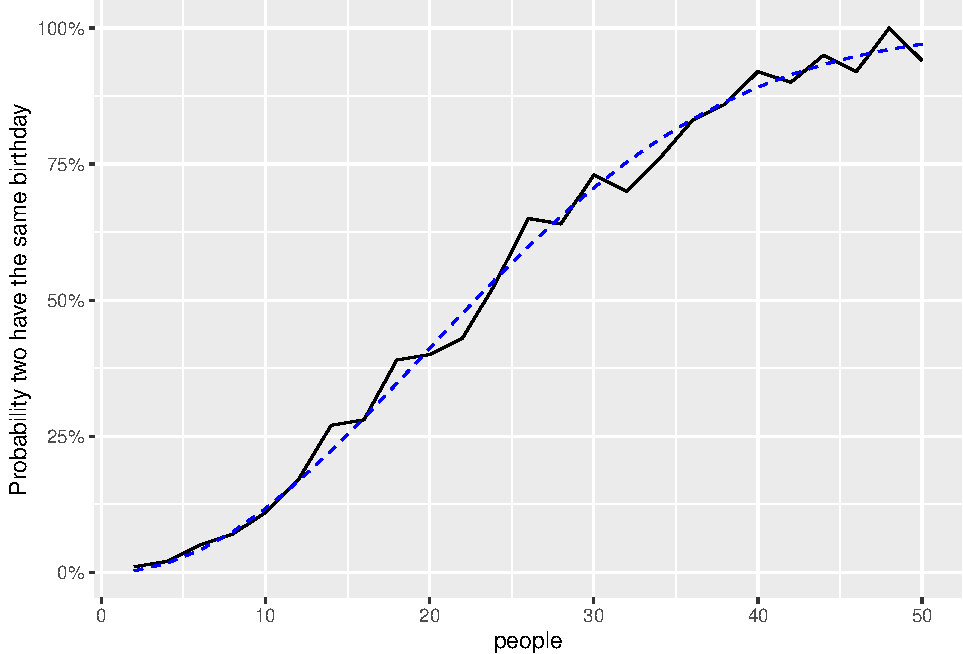
\includegraphics{test-book_files/figure-latex/unnamed-chunk-10-2.pdf}

\begin{Shaded}
\begin{Highlighting}[]
\NormalTok{corrplot}\OperatorTok{::}\KeywordTok{corrplot}\NormalTok{(M, }\DataTypeTok{method =} \StringTok{"color"}\NormalTok{, }\DataTypeTok{type =} \StringTok{"upper"}\NormalTok{)}
\end{Highlighting}
\end{Shaded}

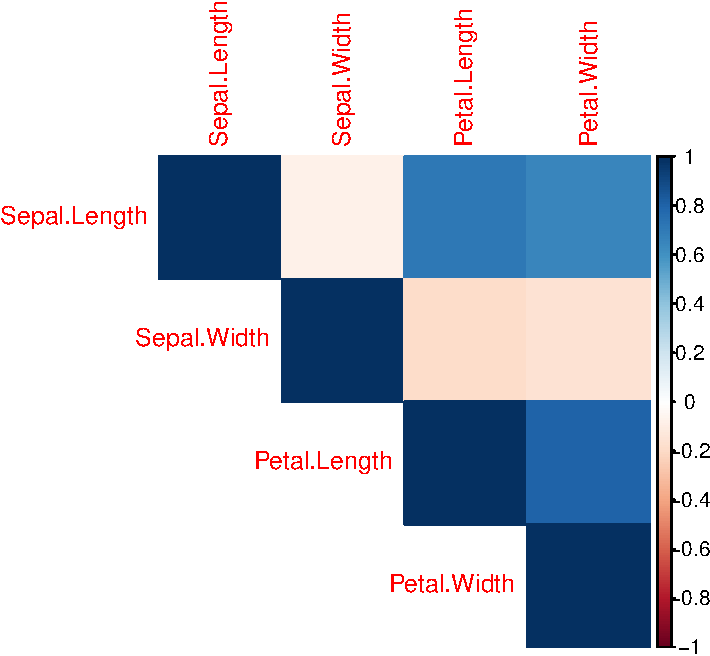
\includegraphics{test-book_files/figure-latex/unnamed-chunk-10-3.pdf}

\begin{Shaded}
\begin{Highlighting}[]
\NormalTok{corrplot}\OperatorTok{::}\KeywordTok{corrplot}\NormalTok{(M, }\DataTypeTok{method =} \StringTok{"color"}\NormalTok{, }\DataTypeTok{type =} \StringTok{"upper"}\NormalTok{, }\DataTypeTok{order =} \StringTok{"hclust"}\NormalTok{)}
\end{Highlighting}
\end{Shaded}

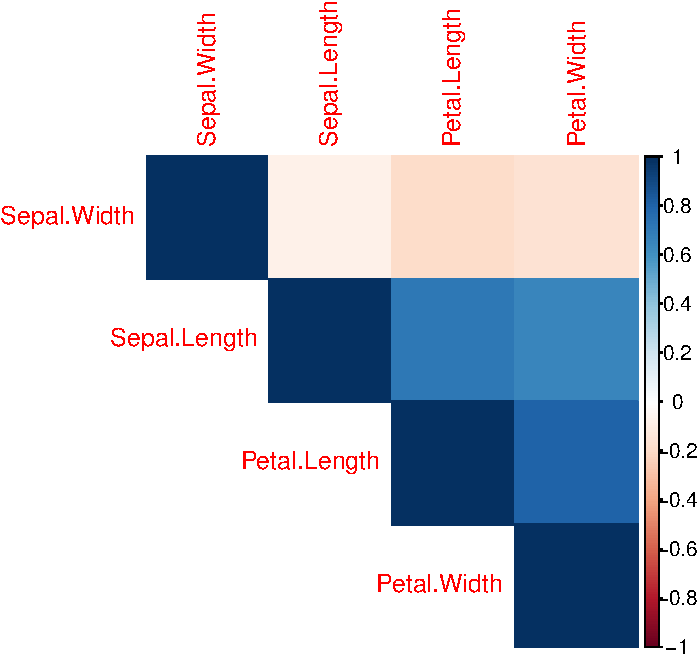
\includegraphics{test-book_files/figure-latex/unnamed-chunk-10-4.pdf}

\begin{Shaded}
\begin{Highlighting}[]
\NormalTok{corrplot}\OperatorTok{::}\KeywordTok{corrplot}\NormalTok{(M, }\DataTypeTok{method =} \StringTok{"color"}\NormalTok{, }\DataTypeTok{type =} \StringTok{"upper"}\NormalTok{, }\DataTypeTok{order =} \StringTok{"hclust"}\NormalTok{, }\DataTypeTok{addCoef.col =} \StringTok{"black"}\NormalTok{)}
\end{Highlighting}
\end{Shaded}

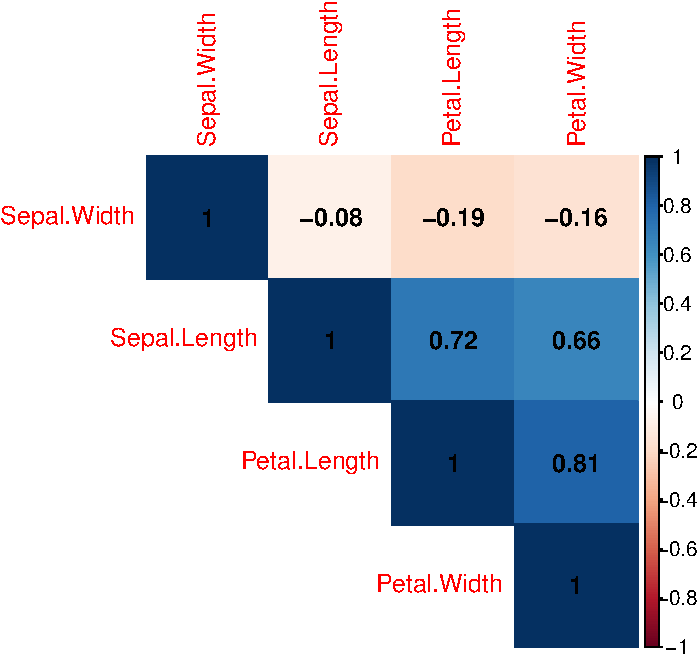
\includegraphics{test-book_files/figure-latex/unnamed-chunk-10-5.pdf}

\begin{Shaded}
\begin{Highlighting}[]
\NormalTok{corrplot}\OperatorTok{::}\KeywordTok{corrplot}\NormalTok{(M, }\DataTypeTok{method =} \StringTok{"color"}\NormalTok{, }\DataTypeTok{type =} \StringTok{"upper"}\NormalTok{, }\DataTypeTok{order =} \StringTok{"hclust"}\NormalTok{, }\DataTypeTok{addCoef.col =} \StringTok{"black"}\NormalTok{, }\DataTypeTok{tl.col=}\StringTok{"black"}\NormalTok{)}
\end{Highlighting}
\end{Shaded}

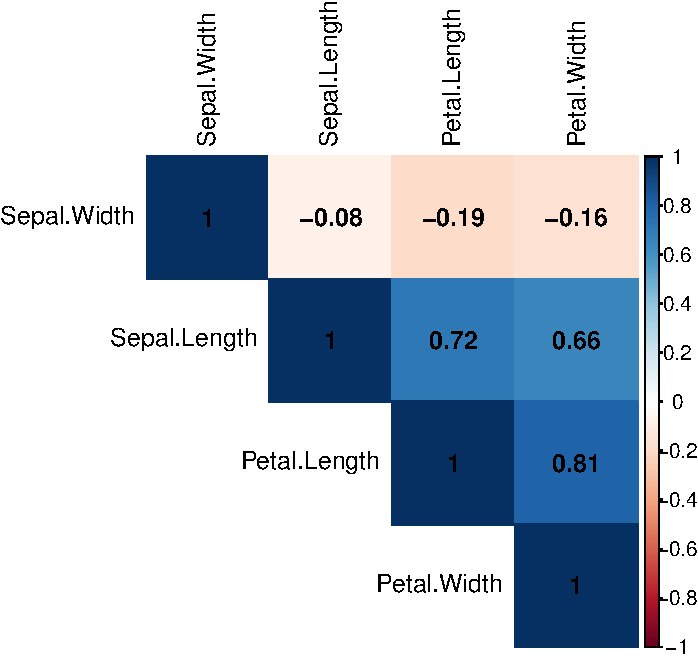
\includegraphics{test-book_files/figure-latex/unnamed-chunk-10-6.pdf}

\begin{Shaded}
\begin{Highlighting}[]
\NormalTok{corrplot}\OperatorTok{::}\KeywordTok{corrplot}\NormalTok{(M, }\DataTypeTok{method =} \StringTok{"color"}\NormalTok{, }\DataTypeTok{type =} \StringTok{"upper"}\NormalTok{, }\DataTypeTok{order =} \StringTok{"hclust"}\NormalTok{, }\DataTypeTok{addCoef.col =} \StringTok{"black"}\NormalTok{, }\DataTypeTok{tl.col=}\StringTok{"black"}\NormalTok{, }\DataTypeTok{tl.srt =} \DecValTok{45}\NormalTok{)}
\end{Highlighting}
\end{Shaded}

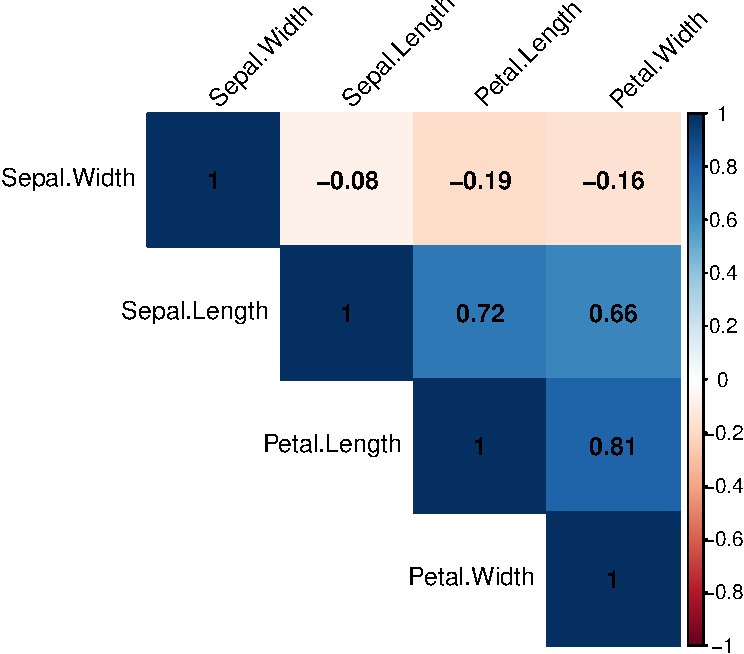
\includegraphics{test-book_files/figure-latex/unnamed-chunk-10-7.pdf}

\hypertarget{ifelsecasewhen}{%
\chapter{if\_else() and case\_when(): Comparison}\label{ifelsecasewhen}}

\hypertarget{case_when}{%
\section{case\_when()}\label{case_when}}

case\_when() from \url{https://www.rdocumentation.org/packages/dplyr/versions/0.7.8/topics/case_when}

\begin{Shaded}
\begin{Highlighting}[]
\NormalTok{x <-}\StringTok{ }\DecValTok{1}\OperatorTok{:}\DecValTok{50}
\NormalTok{y <-}\StringTok{ }\DecValTok{51}\OperatorTok{:}\DecValTok{100}

\NormalTok{df <-}\StringTok{ }\KeywordTok{data.frame}\NormalTok{(x,y)}
\NormalTok{df}
\end{Highlighting}
\end{Shaded}

\begin{verbatim}
##     x   y
## 1   1  51
## 2   2  52
## 3   3  53
## 4   4  54
## 5   5  55
## 6   6  56
## 7   7  57
## 8   8  58
## 9   9  59
## 10 10  60
## 11 11  61
## 12 12  62
## 13 13  63
## 14 14  64
## 15 15  65
## 16 16  66
## 17 17  67
## 18 18  68
## 19 19  69
## 20 20  70
## 21 21  71
## 22 22  72
## 23 23  73
## 24 24  74
## 25 25  75
## 26 26  76
## 27 27  77
## 28 28  78
## 29 29  79
## 30 30  80
## 31 31  81
## 32 32  82
## 33 33  83
## 34 34  84
## 35 35  85
## 36 36  86
## 37 37  87
## 38 38  88
## 39 39  89
## 40 40  90
## 41 41  91
## 42 42  92
## 43 43  93
## 44 44  94
## 45 45  95
## 46 46  96
## 47 47  97
## 48 48  98
## 49 49  99
## 50 50 100
\end{verbatim}

\begin{Shaded}
\begin{Highlighting}[]
\KeywordTok{case_when}\NormalTok{(}
\NormalTok{  x }\OperatorTok\StringTok{ }\DecValTok{35} \OperatorTok{==}\StringTok{ }\DecValTok{0} \OperatorTok{~}\StringTok{ "fizz buzz"}\NormalTok{,}
\NormalTok{  x }\OperatorTok\StringTok{ }\DecValTok{5} \OperatorTok{==}\StringTok{ }\DecValTok{0} \OperatorTok{~}\StringTok{ "fizz"}\NormalTok{,}
\NormalTok{  x }\OperatorTok\StringTok{ }\DecValTok{7} \OperatorTok{==}\StringTok{ }\DecValTok{0} \OperatorTok{~}\StringTok{ "buzz"}\NormalTok{,}
  \OtherTok{TRUE} \OperatorTok{~}\StringTok{ }\KeywordTok{as.character}\NormalTok{(x)}
\NormalTok{)}
\end{Highlighting}
\end{Shaded}

\begin{verbatim}
##  [1] "1"         "2"         "3"         "4"         "fizz"      "6"        
##  [7] "buzz"      "8"         "9"         "fizz"      "11"        "12"       
## [13] "13"        "buzz"      "fizz"      "16"        "17"        "18"       
## [19] "19"        "fizz"      "buzz"      "22"        "23"        "24"       
## [25] "fizz"      "26"        "27"        "buzz"      "29"        "fizz"     
## [31] "31"        "32"        "33"        "34"        "fizz buzz" "36"       
## [37] "37"        "38"        "39"        "fizz"      "41"        "buzz"     
## [43] "43"        "44"        "fizz"      "46"        "47"        "48"       
## [49] "buzz"      "fizz"
\end{verbatim}

\hypertarget{compare-this-with-if_else}{%
\section{Compare this with if\_else()}\label{compare-this-with-if_else}}

\begin{Shaded}
\begin{Highlighting}[]
\KeywordTok{if_else}\NormalTok{(x }\OperatorTok\StringTok{ }\DecValTok{2} \OperatorTok{==}\StringTok{ }\DecValTok{0}\NormalTok{, }\StringTok{"even"}\NormalTok{, }\StringTok{"odd"}\NormalTok{)}
\end{Highlighting}
\end{Shaded}

\begin{verbatim}
##  [1] "odd"  "even" "odd"  "even" "odd"  "even" "odd"  "even" "odd"  "even"
## [11] "odd"  "even" "odd"  "even" "odd"  "even" "odd"  "even" "odd"  "even"
## [21] "odd"  "even" "odd"  "even" "odd"  "even" "odd"  "even" "odd"  "even"
## [31] "odd"  "even" "odd"  "even" "odd"  "even" "odd"  "even" "odd"  "even"
## [41] "odd"  "even" "odd"  "even" "odd"  "even" "odd"  "even" "odd"  "even"
\end{verbatim}

\hypertarget{subset}{%
\chapter{Subsetting}\label{subset}}

From \url{https://www.r-bloggers.com/5-ways-to-subset-a-data-frame-in-r/}

Note: since this is down for maintenance, I will turn off evaluation on these chunks:

\begin{Shaded}
\begin{Highlighting}[]
\NormalTok{education <-}\StringTok{ }\KeywordTok{read.csv}\NormalTok{(}\StringTok{"https://vincentarelbundock.github.io/Rdatasets/csv/robustbase/education.csv"}\NormalTok{, }\DataTypeTok{stringsAsFactors =} \OtherTok{FALSE}\NormalTok{)}

\KeywordTok{colnames}\NormalTok{(education) <-}\StringTok{ }\KeywordTok{c}\NormalTok{(}\StringTok{"X"}\NormalTok{,}\StringTok{"State"}\NormalTok{,}\StringTok{"Region"}\NormalTok{,}\StringTok{"Urban.Population"}\NormalTok{,}\StringTok{"Per.Capita.Income"}\NormalTok{,}\StringTok{"Minor.Population"}\NormalTok{,}\StringTok{"Education.Expenditures"}\NormalTok{)}

\KeywordTok{glimpse}\NormalTok{(education)}
\end{Highlighting}
\end{Shaded}

\begin{verbatim}
## Rows: 50
## Columns: 7
## $ X                      <int> 1, 2, 3, 4, 5, 6, 7, 8, 9, 10, 11, 12, 13, 1...
## $ State                  <chr> "ME", "NH", "VT", "MA", "RI", "CT", "NY", "N...
## $ Region                 <int> 1, 1, 1, 1, 1, 1, 1, 1, 1, 2, 2, 2, 2, 2, 2,...
## $ Urban.Population       <int> 508, 564, 322, 846, 871, 774, 856, 889, 715,...
## $ Per.Capita.Income      <int> 3944, 4578, 4011, 5233, 4780, 5889, 5663, 57...
## $ Minor.Population       <int> 325, 323, 328, 305, 303, 307, 301, 310, 300,...
## $ Education.Expenditures <int> 235, 231, 270, 261, 300, 317, 387, 285, 300,...
\end{verbatim}

\hypertarget{subsetting-using-brackets}{%
\section{Subsetting using brackets}\label{subsetting-using-brackets}}

\begin{Shaded}
\begin{Highlighting}[]
\NormalTok{education[}\KeywordTok{c}\NormalTok{(}\DecValTok{10}\OperatorTok{:}\DecValTok{21}\NormalTok{),}\KeywordTok{c}\NormalTok{(}\DecValTok{2}\NormalTok{,}\DecValTok{6}\OperatorTok{:}\DecValTok{7}\NormalTok{)]}
\end{Highlighting}
\end{Shaded}

\begin{verbatim}
##    State Minor.Population Education.Expenditures
## 10    OH              324                    221
## 11    IN              329                    264
## 12    IL              320                    308
## 13    MI              337                    379
## 14    WI              328                    342
## 15    MN              330                    378
## 16    IA              318                    232
## 17    MO              309                    231
## 18    ND              333                    246
## 19    SD              330                    230
## 20    NB              318                    268
## 21    KS              304                    337
\end{verbatim}

\hypertarget{subset-using-brackets-by-omitting-the-rows-and-columns-we-dont-want}{%
\section{Subset using brackets by omitting the rows and columns we don't want}\label{subset-using-brackets-by-omitting-the-rows-and-columns-we-dont-want}}

\begin{Shaded}
\begin{Highlighting}[]
\NormalTok{education[}\OperatorTok{-}\KeywordTok{c}\NormalTok{(}\DecValTok{1}\OperatorTok{:}\DecValTok{9}\NormalTok{,}\DecValTok{22}\OperatorTok{:}\DecValTok{50}\NormalTok{),}\OperatorTok{-}\KeywordTok{c}\NormalTok{(}\DecValTok{1}\NormalTok{,}\DecValTok{3}\OperatorTok{:}\DecValTok{5}\NormalTok{)]}
\end{Highlighting}
\end{Shaded}

\begin{verbatim}
##    State Minor.Population Education.Expenditures
## 10    OH              324                    221
## 11    IN              329                    264
## 12    IL              320                    308
## 13    MI              337                    379
## 14    WI              328                    342
## 15    MN              330                    378
## 16    IA              318                    232
## 17    MO              309                    231
## 18    ND              333                    246
## 19    SD              330                    230
## 20    NB              318                    268
## 21    KS              304                    337
\end{verbatim}

\hypertarget{subset-using-brackets-in-combination-with-the-which-function-and-the-in-operator}{%
\section{Subset using brackets in combination with the which() function and the \%in\% operator}\label{subset-using-brackets-in-combination-with-the-which-function-and-the-in-operator}}

\begin{Shaded}
\begin{Highlighting}[]
\NormalTok{education[}\KeywordTok{which}\NormalTok{(education}\OperatorTok{$}\NormalTok{Region }\OperatorTok{==}\StringTok{ }\DecValTok{2}\NormalTok{),}\KeywordTok{names}\NormalTok{(education) }\OperatorTok\StringTok{ }\KeywordTok{c}\NormalTok{(}\StringTok{"State"}\NormalTok{,}\StringTok{"Minor.Population"}\NormalTok{,}\StringTok{"Education.Expenditures"}\NormalTok{)]}
\end{Highlighting}
\end{Shaded}

\begin{verbatim}
##    State Minor.Population Education.Expenditures
## 10    OH              324                    221
## 11    IN              329                    264
## 12    IL              320                    308
## 13    MI              337                    379
## 14    WI              328                    342
## 15    MN              330                    378
## 16    IA              318                    232
## 17    MO              309                    231
## 18    ND              333                    246
## 19    SD              330                    230
## 20    NB              318                    268
## 21    KS              304                    337
\end{verbatim}

\hypertarget{subset-using-the-subset-function}{%
\section{Subset using the subset() function}\label{subset-using-the-subset-function}}

\begin{Shaded}
\begin{Highlighting}[]
\KeywordTok{subset}\NormalTok{(education, Region }\OperatorTok{==}\StringTok{ }\DecValTok{2}\NormalTok{, }\DataTypeTok{select =} \KeywordTok{c}\NormalTok{(}\StringTok{"State"}\NormalTok{,}\StringTok{"Minor.Population"}\NormalTok{,}\StringTok{"Education.Expenditures"}\NormalTok{))}
\end{Highlighting}
\end{Shaded}

\begin{verbatim}
##    State Minor.Population Education.Expenditures
## 10    OH              324                    221
## 11    IN              329                    264
## 12    IL              320                    308
## 13    MI              337                    379
## 14    WI              328                    342
## 15    MN              330                    378
## 16    IA              318                    232
## 17    MO              309                    231
## 18    ND              333                    246
## 19    SD              330                    230
## 20    NB              318                    268
## 21    KS              304                    337
\end{verbatim}

\hypertarget{subset-using-dyplyrs-filter-and-select}{%
\section{Subset using dyplyr's filter() and select()}\label{subset-using-dyplyrs-filter-and-select}}

\begin{Shaded}
\begin{Highlighting}[]
\KeywordTok{select}\NormalTok{(}\KeywordTok{filter}\NormalTok{(education, Region }\OperatorTok{==}\StringTok{ }\DecValTok{2}\NormalTok{),}\KeywordTok{c}\NormalTok{(State,Minor.Population}\OperatorTok{:}\NormalTok{Education.Expenditures))}
\end{Highlighting}
\end{Shaded}

\begin{verbatim}
##    State Minor.Population Education.Expenditures
## 1     OH              324                    221
## 2     IN              329                    264
## 3     IL              320                    308
## 4     MI              337                    379
## 5     WI              328                    342
## 6     MN              330                    378
## 7     IA              318                    232
## 8     MO              309                    231
## 9     ND              333                    246
## 10    SD              330                    230
## 11    NB              318                    268
## 12    KS              304                    337
\end{verbatim}

\bibliography{book.bib,packages.bib}

\end{document}
